\documentclass{acm_proc_article-sp}

\usepackage{graphicx} %package to manage images
\graphicspath{ {images/} }

\usepackage[rightcaption]{sidecap}

\usepackage{wrapfig}

\begin{document}

\title{Project: Seismic Data Analysis with Spark and MongoDB}

\numberofauthors{4} 
\author{
\alignauthor
Xu Liu\titlenote{PhD student at Indiana University}\\
       \affaddr{Indiana University}\\
       \affaddr{Bloomington, IN}\\
\email{xl41@indiana.edu futuresystems: xl41
Chameleon: xl41}
}

\date{30 September 2016}


\maketitle
\begin{abstract}
We propose to deploy a seismic data processing environment with no-relational database (MongoDB) and Spark. We propose to use tools like Ambari or Ansible to ease the deployment job for Spark cluster.
\end{abstract}

\keywords{Seismology, MongoDB, Spark} % NOT required for Proceedings

\section{Introduction}

The science of seismology is awash in data. In the past 20 years the quantity of data available for the typical seismology research project has grown by at least three orders of magnitude.  Our field is well fed by Incorporated Research Institutions for Seismology (IRIS~\cite{IRIS}) that has done a fantastic job of building and maintaining an accessible archive of these data.  The problem this project addresses, in fact, would not exist were it not for the ready availability of this sea of data from IRIS.  The fundamental community problem this project addresses is that while the available data has grown by many orders of magnitude there have been no major software innovations for processing this ocean of data.  All the standard software tools used by the research community are founding on computing concepts that were leading edge ideas twenty (Antelope~\cite{Antelope}) to thirty (Seismic Analysis Code) years or more ago.  The key premise of this proposal is that this creaky infrastructure is seriously limiting scientific advances in seismology and has imposed a throttle on scientific advances from Earthscope.  The seismology community is like a group of young children given access to the Library of Congress.  We can only read and use a tiny fraction of the information in this vast pile of new data.  

A second principle is that the project proposed here is the engineering part of a strategic research project to address two elements needed to build a more scalable advanced processing system for seismology: (1) a metadata handling system for data processing that is flexible, extensible, and capable of storing the full range ancillary parameters that define a data processing flow, and (2) a scalable, approachable system for implementing algorithms in the modern world of high performance computing characterized by massively parallel systems.


\section{Proposal}

The focus of this project is research to consider the efficacy of two technologies for improving passive array data processing:
1.	The seismic data processing flow in Figure 1 is a typical example of an embarrassingly parallel problem.  The reason is that with this data flow model each seismogram or group (ensemble) of seismograms is processed by the same chain of algorithms each defined by the same set of control parameters.  This type of problem is known to be well suited to the concept of MapReduce as implemented in software packages like Hadoop and Spark.  

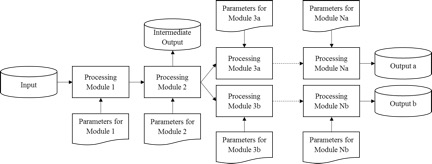
\includegraphics[scale=0.5]{Picture1}

Figure 1 Generic workflow for processing of seismic reflection data.  The workflow commonly begins with the input of raw data and ends with the output of processed results.  The processing modules represent one component of processing such as deconvolution, velocity analysis and migration.  Each processing module is independent, because the input and output conform a predefined format.  Therefore, the intermediate result of each module could be saved and retrieved later.  Most systems provide a means to fork into multiple work flows.  

2.	We propose to use a NoSQL database (MongoDB) as the framework to handle all metadata related to a collection of seismograms.  The idea is to use a common NoSQL database to manage not just conventional header information, but also input parameters for all processes and log information from each processing module. 

For implementation detail of this project, there will be three parts:
Seismic data includes metadata and waveforms, while metadata is stored and managed by Antelope and waveforms are stored on the file system. The data set will be downloaded from USArray, IRIS. The waveforms are encrypted as structured binary files called MiniSEED ~\cite{MiniSeed}. The files need to be loaded into Antelope and file system. This phase needs estimate 1 to 2 weeks, which is expected to be done before Oct. 9th.

To extract, transfer and load the seismic data from Antelope to MongoDB, tool needs to be developed to use the Antelope Python API to read and manipulate the metadata from Antelope and ObsPy~\cite{ObsPy} to read and decrypt the MiniSEED file from the file system and extract the waveforms from them. In order to store all the information, PyMongo~\cite{PyMongo} (MongoDB Python API) will be used to access MongoDB and pickle (Python object serialization) will be used to serialize the seismic waveform data so they can be stored in GridFS, another component for storage within MongoDB. This phase needs estimate 2 weeks, which is expected to be done before Oct. 23rd.

After the data migration from Antelope to MongoDB, Spark must be deployed. For Spark cluster, I plan to deploy three nodes. Ambari~\cite{AboutAmbari} (or Ansible~\cite{Ansible}) will be used to help me manage it. The Apache Ambari project is aimed at making Hadoop management simpler by developing software for provisioning, managing, and monitoring Apache Hadoop clusters. Ambari provides an intuitive, easy-to-use Spark management web UI backed by its RESTful APIs. This phase needs estimate 2 weeks, which is expected to be done before Nov. 6th.
 
After the environment is set, I will deploy sharding for MongoDB to have a better data scalability. Futhermore, I will run some simple DSP algorithms like filtering, downsampling etc. If things goes smoothly, I will try to virtualize the processed seismic data with D3JS at the end of this semester.


\section{Artifacts}
Code on Gitlab
Jupyter Notebook
An Antelope Node or a document to create an Antelope node
A MongoDB Cluster or a document to create a MongoDB cluster
A Spark Cluster or a document to create a Spark cluster
Seismic Data visualization and more if time permits

\bibliographystyle{abbrv}
\bibliography{proposal}

%\balancecolumns 

\end{document}

